\chapter{Implementation}

\setcounter{section}{5}
\setcounter{subsection}{0}

In order to test how well the architecture would perform an implementation is needed. The framework is implemented in Javascript as described in section \ref{sec:architecture}. To be able to discuss the implementation further on in the thesis a name is needed. The implementation will further on be referred to as MinimaJS.

\subsection{Classes and inheritance}

Since the architecture is based on modules that all have different properties a class implementation that has a good support for inheritance would be needed. Unfortunately Javascript is using a prototype-based inheritance model with a limited support for inheritance. Even though there is no native support for traditional inheritance the behavior can be emulated, and there are a number of implementations available for this purpose. One of the more popular implementations is written by John Resig, the founder of jQuery. His implementation is based on the models Base2 and Prototype \cite{john_resig_model}. However, all these models have a behavior that strictly inhibits the traditional inheritance model, but instead have more of a prototype-based approach. Listing \ref{inheritance_shared_obj} shows an example of this behavior. As seen in the example c2.obj.counter is set to 1 but the expected behavior in a traditional inheritance model would be 0. This is the case since objects in Javascript are evaluated with a call-by-reference approach while other primitive datatypes such as integers are evaluated with call-by-value.

\lstset{frame=single, caption=Inheritance using John Resig's inheritance model with shared objects between instances, label=inheritance_shared_obj, captionpos=b, tabsize=2}
\begin{framed}
\begin{lstlisting}
var Parent = Class.extend({
	counter : 0,
	obj : { counter : 0 },
	inca : function() {
		this.counter++;
		this.obj.counter++;
	}
});
var Child = Parent.extend({});

var c1 = new Child();
var c2 = new Child();

c1.inca();

// Prints 1, 1
console.log(c1.counter + ", " + c1.obj.counter);

// Prints 0, 1
console.log(c2.counter + ", " + c2.obj.counter); 
\end{lstlisting}
\end{framed}

In a prototype-based inheritance model a parent instance is shared among all the children. If an object is changed in the parent all children are affected. To get around this each child instance can have its own parent instance. A change in a parent would then only affect one single child, just as expected in a traditional inheritance model. The drawback is of course that it will require more memory to run since there now are more instances stored in the memory. There is no perfect solution to get around this, it is rather a give-and-take situation. If it is important for the design to have a traditional strict inheritance model will it simply require more memory to run, if this is not the case the prototype-based solution should of course be used. Since class inheritance is a crucial part of the system design for MinimaJS, it is based on the solution where each child has its own parent instance.

\subsection{Scopes in Javascript}

All functions in Javascript are executed on a scope. The scope is accessible through the variable {\em this}. The scope can be very handy, for example in a class method {\em this} would typically refer to the current instance of the class. However, due to the nature of Javascript, the code is often written in an event-driven architecture which encourages usage of anonymous functions as callbacks. Whenever these callbacks are fired the scope is changed and {\em this} is replaced with another object. It is on the other hand possible to control what scope a certain function should be fired on, this can be done with the functions {\em call} and {\em apply}. MinimaJS is implemented in a way that tries to maintain the same scope in all possible cases so that the developer does not have to think about its current state. Unfortunately it is in some cases impossible to keep the current scope, a Javascript-developer must always think about when the scope may change.

\subsection{API drivers and push synchronization}

Two different kind of API drivers were implemented, one for local storage and one for storage on a server. The API driver for local storage on a client is based on the Local Storage API in the HTML5 draft which allows strings to be permanently stored on a client. By serializing data to JSON more complex objects can be stored as well. The other API driver is based on websockets which also comes from the HTML5 draft. Websockets support bidirectional communication between the client and the server \cite{websocket_draft}. This API driver fully support synchronization between several clients simultaneously.

When several clients are using the system at the same time synchronization problems may appear. These problems appear whenever two clients are doing concurrent transactions against the database. Other more organizational problems may also appear if the users are working with data that is out-of-date, the users might take decisions that is based on the old set of data. These problems can be approached by introducing a protocol for synchronization that is implemented within the API driver. The purpose of the protocol is to allow changes to be distributed among all the clients so that conflicts can be detected and resolved. Each model object is tagged with a revision, when a change is made on the model the revision is increased. The server can detect when a change is made to an old revision and tell this to the client sending the change since this corresponds to a conflict. Whenever a client sends a change request on a model the server will respond with an ack or nack depending on if the change was carried through or not. The API driver must be able to both commit and revert changes on a model. In order to get a good user experience a model is locally changed directly when the user makes a change, first when the model is saved the transaction is sent to the server. The view will therefore be re-rendered directly which results in a more responsive system. When the server answers the transaction will either be committed or reverted depending on if the answer was an ack or nack. In order to get a more simple protocol a synchronous message passing is used, a client is only allowed to send one transaction at a time. Once a client has sent a change to the server must it wait until an ack or nack is received before sending another one. This was implemented using a queue of transactions. An illustration of how the protocol was designed can be seen in figure \ref{fig:sync}. The figure shows when client {\em i} has made two changes that are sent to the server. The server accepts the first change and answers with an ack, the seconds change is however out-of-date and is therefore rejected with a nack. All other clients, except for {\em i} itself, are notified by the first change that was carried through.

\begin{figure}[h!]
	\centerline{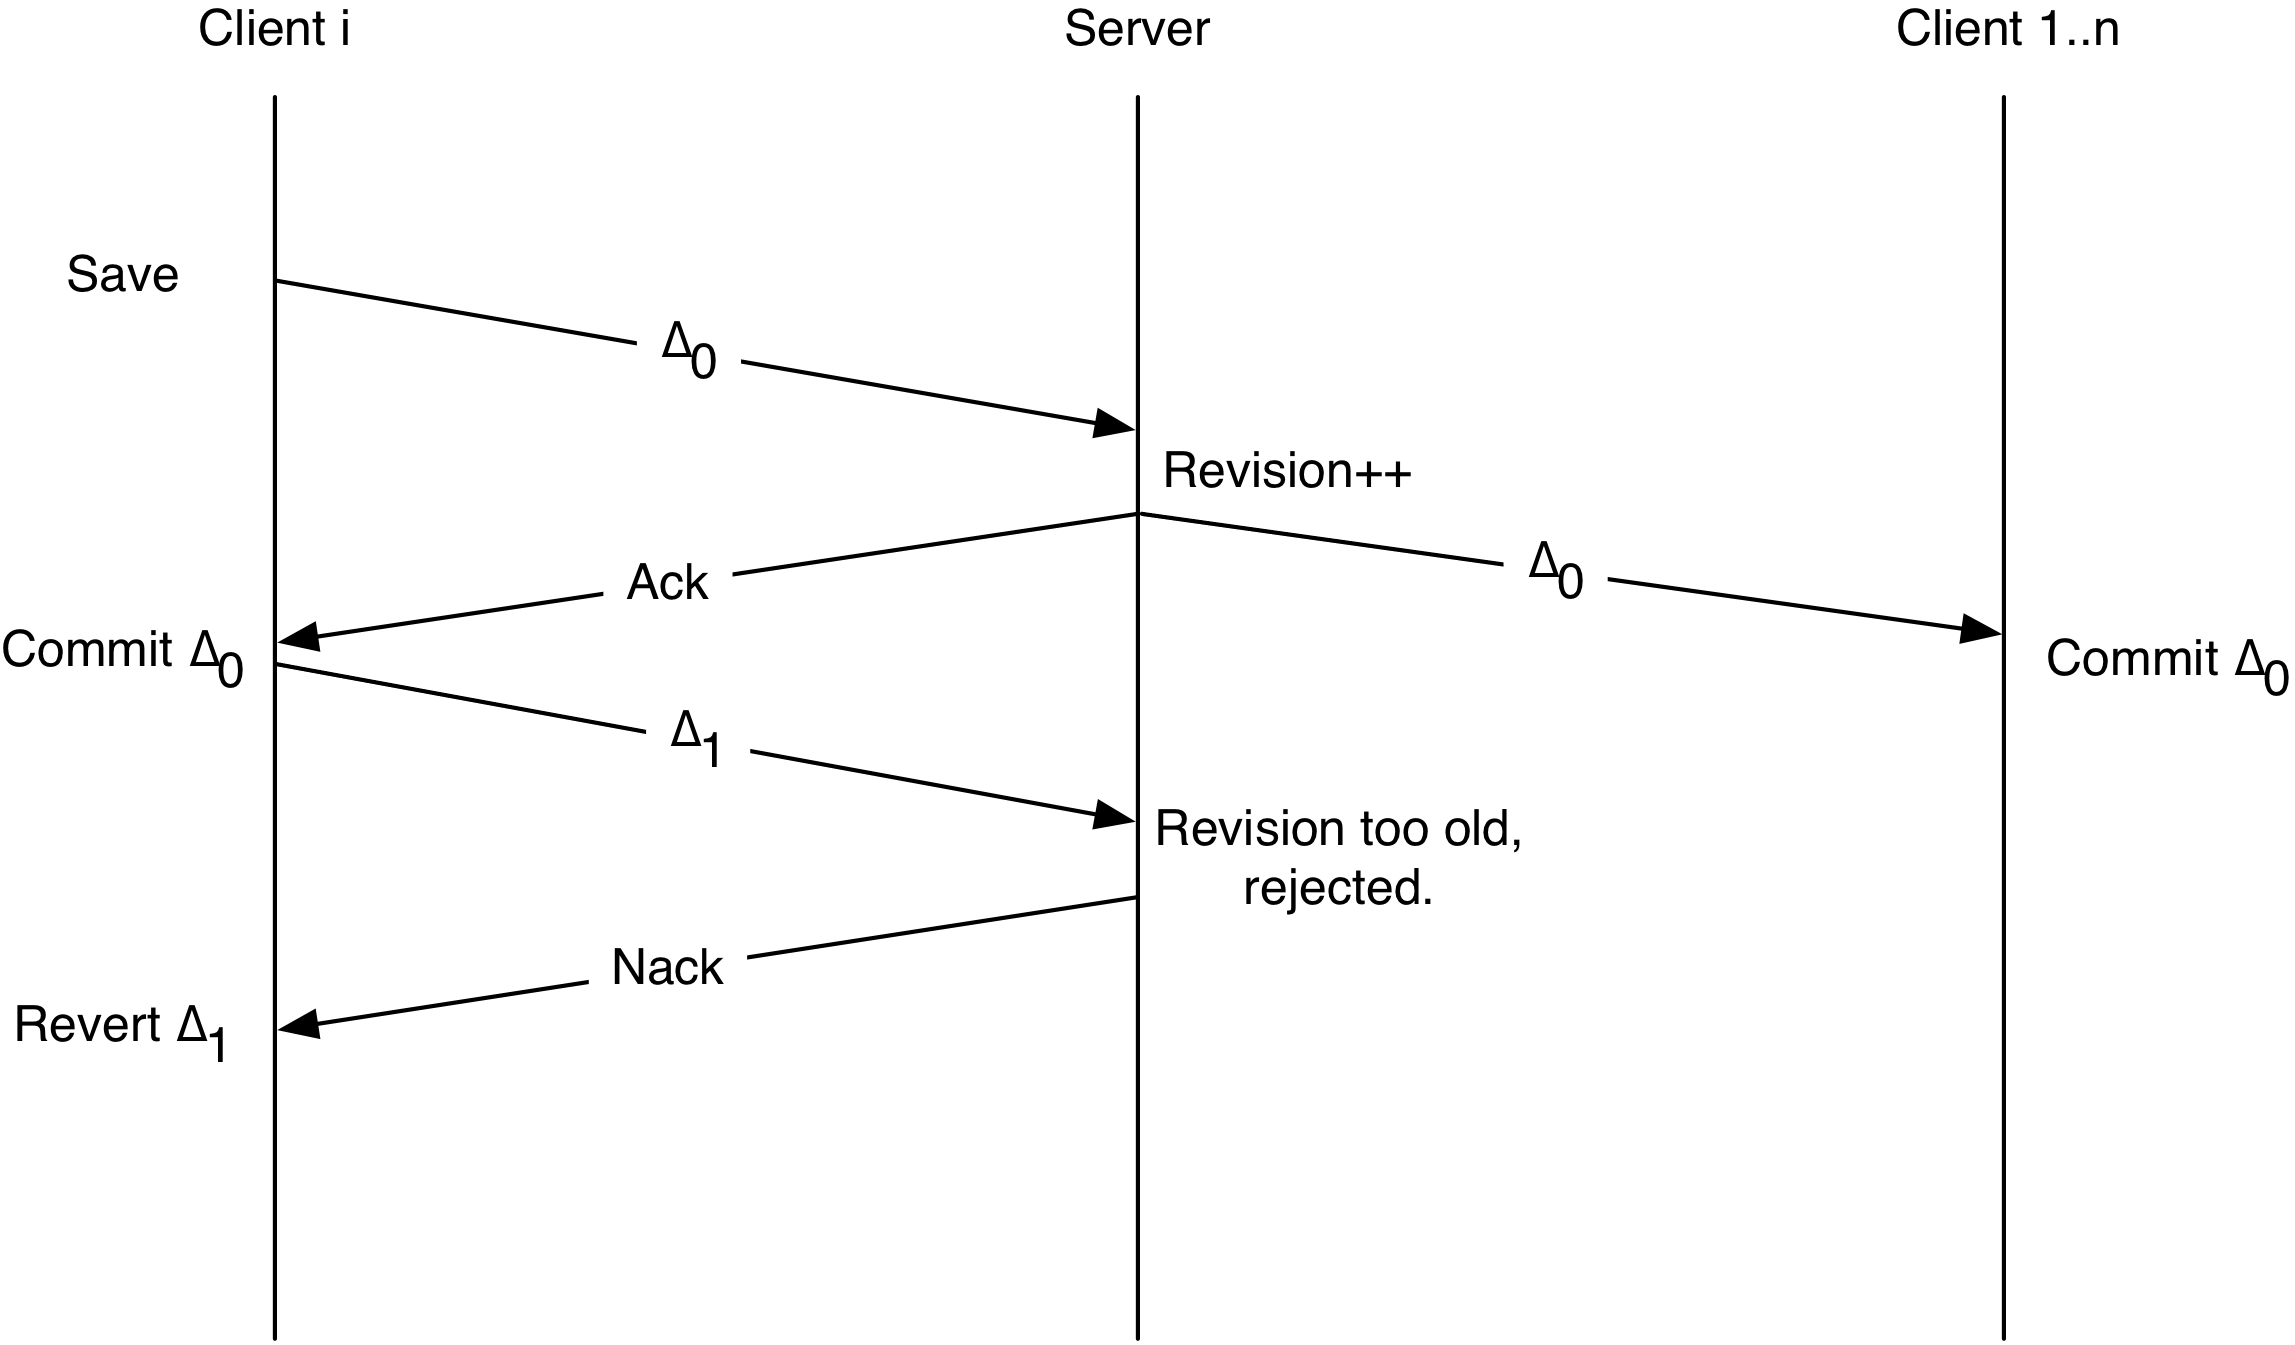
\includegraphics[width=120mm]{gfx/sync.png}}
	\caption{An illustration of a client sending two changes to the server.}
	\label{fig:sync}
\end{figure}

\subsection{Writing testable code}

By letting the presentation models be accessible from the module's instance unit tests can be written without interacting with the user interface. Most of the features of the application can then be tested during development with small and simple unit tests. Important to note is that if the unit tests do not interact with the user interface the views would not be tested. On the other hand it will encourage developers to write simple, almost trivial, views that only present the data that its given. A unit test can emulate user input by sending the same event to the controller as the presentation model would do. The result can then be verified by either looking directly at the affected models or listening to events sent by the collection. Every time a view is rendered an event is also sent, by listening to these events the unit test can verify that the correct views are rendered. The unit tests can then validate that the correct data was set and that the right views were rendered. This provides a good basis for a working application.

\subsection{Dependencies}

MinimaJS has two hard dependencies, one template engine, one selector library. In order to keep the file size low these dependencies are configurable. For example, if jQuery is already used on the site MinimaJS can be configured to use jQuery as its selector library. It would be a waste to include the jQuery library twice. In other cases where jQuery is not used on the site other more lightweight alternatives can be used, such as Sizzle. When it comes to template engines there are several alternatives, each alternative has of course its own advantages and disadvantages. Depending on the application some template languages might be more suitable than others. The template engine can, just as the selector library, be specified in the configuration. At last, the API drivers depend on the JSON library by Douglas Crockford \cite{json} for the serialization/deserialization of the data models.

\subsection{Javascript render API for SEO}

As explained in section \ref{sec:seo_a_new_approach} an API that can render and run the Javascript on a given site is needed. The API is implemented using PhantomJS to render the given page. PhantomJS is a headless webkit browser with an excellent support for Javascript that can be run in a server-side environment. For the API to know when all the asynchronous requests are finished two different triggers can be used, either a DOM-element or a flag can be specified. If a DOM-element is used as trigger the site is considered as completely loaded once this element is updated with some content. The DOM-element is simply polled periodically to check if it has been updated. When instead a frag is used as trigger it is simply polled until a truthy value appears. What type of trigger that is used is set in the Javascript on the site which makes it a quite flexible solution since different pages can use different triggers. If caching is used it will depend on the backend system. In order to test the SEO implementation with cache it was implemented in PHP using MySQL as backend storage.

\subsection{Deployment}

To minimize the time it takes for a client to download and parse the Javascript a number of actions can be performed. These actions will all together decrease the time it takes before the page can be rendered at the client.

Each time a new TCP connection opens a handshake is performed \cite{tcp_handshake}. The speed is limited by TCP's congestion control which limits the window size. The size of the window is then increased over time until a packet is dropped \cite{tcp_congestion_control}. The connection is therefore quite slow in the beginning. Since it is likely that an application consists of dozens of Javascript files the total download time will be affected by how new connections are handled in TCP. On top of that are browsers limiting the number of concurrent TCP connections. For example is Google Chrome currently limited to 6 concurrent connections. By concatenating the Javascript files together fewer TCP connections will be opened, and since the window-size grows exponentially over time this will result in a shorter download time in total. Exactly how many files that should be used depends on the application, and tests must be performed to find the optimal number of files for a specific application \cite{concat_files}.

To decrease the file size of the Javascript it can be minified using tools such as UglifyJS, YUI compressor or Closure Compiler. A minifier tool tries to optimize the Javascript code to decrease the file size as much as possible. By changing variable names, removing comments and whitespaces the file size can be decreased, but it is of course important that the functionality is kept intact. Other optimizations that can be done are letting the webserver compress all the files before sending them to the client. The gzip compression has a wide browser support which makes it highly suitable to use for this kind of task, for browsers that do not support gzip instead a non-compressed file can be served. By compressing the files with gzip the response can be reduced by about 70\% \cite{gzip_reduce_size}. The gzip format is based on the deflate algorithm which combines LZ77 and Huffman coding. It simply finds common strings and replaces them with pointers (LZ77). Symbols are then replaced with weighted symbols based on their frequency of use (Huffman coding) \cite{deflate}. This is extra useful for Javascript views that are described in HTML which tend to share long sub-strings. The drawback with compressing the files is that it takes additional CPU cycles to perform which results in a higher load on the web server. On the other hand can the web server cache the compressed files so each file do not have to be compressed at each request.

Another important aspect to consider is DNS lookups. From a lookup perspective it would be ideal if all files were downloaded from the same host that is serving the HTML page. This would minimize the number of lookups since the IP address of the host already is in the DNS cache of the client. If external libraries are used, for example if jQuery is loaded from an external server, CDNs (Content Delivery Networks) should be considered. The idea with a CDN is to distribute data across the internet on servers with high availability and good performance. For example, if a user has visited another site that is using the same CDN for jQuery it is already in the cache of the user and will therefore not be downloaded again. The drawback is that if it is not in the cache of the client another DNS lookup must be performed. The site also becomes dependent on the CDN, if the CDN is not available the entire site will fail to load.

When the frontend becomes big it is sometimes unnecessary to download all the Javascript when the page is loaded since all of the Javascript might not be needed at that specific page. Only the parts that are needed at first are required to be downloaded immediately so that the page can quickly be rendered, the rest of the Javascript can be downloaded asynchronously later on. To know which Javascript files are needed a dependency-tree can be constructed. This describes what other files a given file depends on. For example the page might depend on the framework and the framework itself depends on a number of Javascript libraries, then the page indirectly depends on these libraries. The files can then be divided into and page-specific code and code that is shared between the modules. Tools such as RequireJS can help with the analysis so that the minimum amount of files are fetched synchronously. These tools can be used independently on the implementation, the modules can simply be wrapped into new tool-specific modules which helps the tool to identify the dependencies.
